\section*{Optimizations}

There are different kinds of optimization: Power, Space, Time.

\begin{compactitem}[$\quad\bullet$]
	\item \textbf{Constant Folding}: If operands are statically known, compute value at compile-time. More general \textbf{algebraic simplification}: Use mathematical identities.

	\item \textbf{Constant Propagation}: If $x$ is a constant replace its uses by the constant.

	\item \textbf{Copy Propagation}: For $x = y$ replace uses of $x$ with $y$

	\item \textbf{Dead Code Elimination}: If side-effect free code can never be observed, safe to eliminate it.

	\item \textbf{Inlining}: Replace a function call with the body of the function (arguments are rewritten to local variables).

	\item \textbf{Code Specialization}: Create Specialized versions of a function that is called form different places with different arguments.

	\item \textbf{Common Subexpression Elimination}: It is the opposite of inlining, fold redundant computations together.

	\item \textbf{Loop Optimizations}
	\begin{compactitem}[$\quad\bullet$]
		\item Hot spots often occur in loops (esp. inner loops)
		\item \textbf{Loop Invariant Code Motion} (hoist outside)
		\item \textbf{Strength Reduction} (replace expensive ops by cheap ones by creating a dependent induction variable)
		\item \textbf{Loop Unrolling}
	\end{compactitem}
\end{compactitem} \medskip

\vspace{-15pt}
\begin{center}
	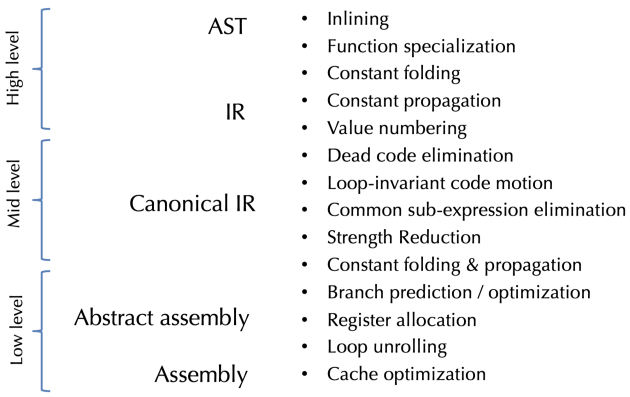
\includegraphics[width=0.9\linewidth]{assets/optimization_diag.png}
\end{center}
\vspace{-10pt}



\subsection*{Dataflow Analysis}

gen[n] := rhs of the exp (if E = "A = B" then gen[n] = B")\\
kill[n] := all exp containing var on LHS (from the prev. example: A)\medskip

Almost every dataflow analysis is a variation of the following algorithm.\smallskip

\textbf{Forward Must Dataflow Analysis}
\begin{lstlisting}
	for all n, in[n] = T, out[n] = T
	repeat until no change in 'in' or 'out'
		for all n
			in[n] = intersect out[n`] for all n` in pred[n]
			out[n] = gen[n] union (in[n] \ kill[n])	
\end{lstlisting}
\textbf{Backward}: swap \texttt{in} and \texttt{out} and \texttt{pred} with \texttt{succ}.
\textbf{May}: swap $\top$ with $\bot$ or $\emptyset$ and replace \textcolor{blue}{\texttt{intersect}} with \textcolor{blue}{\texttt{union}}.\medskip
For each dataflow analysis we only need to define the set \texttt{gen}, \texttt{kill} as well as the domain of dataflow values $\mathcal L$ and a combining operator $\cup$ or $\cap$.\medskip

Most Data-flow analysis follows this template: \\
$\square_1 \ [n] = \ \blacksquare \ _{n' \in \ \square_3 \ [n]} \ \square_2 \ [n']$ \\
$\square_2 \ [n] = gen[n] \cup (\ \square_1 \ [n] \backslash kill[n])$ \\
And the modifications will be: \\
Forward: $\ \square_1 \ = in \ ; \ \ \ \square_2 = out \ ; \ \ \ \square_3 = pred$ \\
Backward: $\ \square_1 \ = out \ ; \ \ \ \square_2 = in \ ; \ \ \ \square_3 = succ$ \\
May: $\ \blacksquare \ = \bigcup$ \\
Must: $\ \blacksquare \ = \bigcap$ \\
\medskip

\textbf{Liveness} (Backward, May)\medskip

We can use the same registers for multiple \texttt{\%uids} if they are not alive at the same time
(\textbf{live[n]} = uids used before end/reassign).
We define \texttt{gen[s]} as all the variables used (RHS) and \texttt{kill[s]} as all the variables defined by statement $s$ (LHS). $\mathcal L$ corresponds to the variables and the combination operator to the set union.\medskip

It holds: in[$n$] $\supseteq$ gen[$n$], in[$n$] $\supseteq$ out[$n$] $\backslash$ kill[$n$] and out[$n$] $\supseteq$ in[$n'$] if $n' \in $ succ[$n$].\medskip

\textbf{Reaching Definition} (Forward, May)\medskip

What variable definitions reach a particular use of a variable? Used for constant and copy propagation.
\texttt{in / out} is the set of nodes defining some variable such that the definition may reach the beginning resp.
end of the current node. For a statement $d_i: A=B:$ we have $d_i \in \textbf{gen[n]}$ and $\textbf{kill[n]}=\{d_i | d_i \ \text{defines same variable} \land d_i \notin gen[n]\} $\medskip

It holds: out[$n$] $\supseteq$ gen[$n$], in[$n$] $\supseteq$ out[$n'$] if $n' \in$ pred[$n$] and out[$n$] $\supseteq$ in[$n$] $\backslash$ kill[$n$] or out[$n$] $\cup$ kill[$n$] $\supseteq$ in[$n$].\medskip

\textbf{Available Expressions} (Forward, Must)\medskip

Used for common subexpression elimination.
\texttt{in / out} are the set of nodes whose values are available on entry / exit of the current node.
For a statement $d_i: A=B:$ we have $d_i \in \textbf{gen[n]} \;\backslash\; \text{kill[n]}$ and $\textbf{kill[n]}=\{d_i | \text{$d_i$ uses A (RHS)}\}$\medskip

\textbf{Very Busy} (Backward, Must)\medskip

An expression is very busy at location $p$, if every path from $p$ must evaluate the expression before any variable is redefined.
It is used for hoisting expressions. \textbf{in/out/gen allow for expressions (x+y)} \medskip

\texttt{gen[B]} = \{expr; expr a op b is evaluated in B, neither a nor b are subsequently redefinded in B \}\smallskip

\texttt{kill[B]} = \{expr; a or b of expr a op b are defined in B and a op b is not subsequently evaluated in B\} \medskip

\textbf{Dominators} (Forward, Must)\medskip

Define \texttt{dom[n]} as the set of all nodes that dominate \texttt{n}, i.e. \texttt{dom[n] = out[n]}, \texttt{gen} is the singelton set of the node itself, \texttt{kill} is the empty set.\medskip

The iterative solution computes the ideal meet-over-path solution if the flow function distributes over $\cap$. Most of the problems that express properties on how the program computes are distributive and compute the MOP solution, analyses of what the program computes do not (e.g. constant propagation). Our analyses also always terminate, as the flow function (\texttt{out[n] = ...}) is monotonic.\medskip

\textbf{Soundness} is defined as an under approximation of the set of variables.


\subsection*{Register Allocation}

\textbf{Linear-Scan Register Allocation}\medskip

Compute liveness information and then scan through the program, for each instruction try to find an available register, else spill it on the stack.\medskip

\textbf{Graph Coloring}\medskip

Compute liveness information for each temp, create an inference graph (nodes are temps and there is an edge if they are alive at the same time), try to color the graph.\medskip

\begin{algorithm}[Kempe's Algorithm]
\begin{verbatim}
    
1) until all nodes deleted: 
   find a node with degree < k and cut it out of the graph
2) recursively k-color the remaining subgraph, 
   when remaining graph is colored, there must be 
   at least one free color available for the deleted node.
3) if the graph cannot be colored, spill a node and retry.
\end{verbatim}
%\begin{compactitem}[$\quad\bullet$]
%    \item 
%	\item Find a node with degree $< k$ and cut it out of the graph
%	\item Recursively $k$-color the remaining subgraph
%	\item When remaining graph is colored, there must be at least one free color available for the deleted %node.
%	\item If the graph cannot be colored we spill a node and try again.
%\end{compactitem}\medskip
\end{algorithm}

\textbf{Optimistic Coloring}
If we get lucky with the choices of colors made earlier, it is sometimes possible to color a
node marked for spilling.\medskip

\textbf{Accessing Spilled Registers:}
If optimistic coloring fails, we need to generate code to move the spilled temporaries to and from memory
\begin{compactitem}
    \item reserve at least 2 regs for moving to/from memory $\Rightarrow$ 2 less regs available to color graph, but coloring only needed once.
    \item Rewrite the program to use a new temporary with explicit move to and from memory. This allows us to reserve fewer register but introduces a change in live ranges, so we must recompute the liveness and recolor the graph.
\end{compactitem}\medskip

\textbf{Coalescing Interference Graphs}
This can be improved by adding \texttt{move} related edges (temps used in a move should have the same color). More aggresively, we may coalesce two move-related nodes into one. This may increase the degree of a node, so we need to be careful. \medskip

\textbf{Brigg}'s strategy is to only coalesce if the resulting node has fewer than $k$ neighbors with degree $\geq k$. \medskip

\textbf{George}'s strategs is to only coalesce if for every neighbor $t$ of one of the coalescing nodes $x$, $t$ also interferes with the other coalescing node or $t$ has degree $< k$.\medskip

In practice we use George’s strategy if one of x and y is precolored and we use Briggs’ strategy if both are temporaries. \medskip

\textbf{Precolored Nodes}: Certain variables must be pre-assigned to regs (\texttt{call}, \texttt{imul}, caller-save registers) e.g. on X86 imul must define \%rax. To properly allocate temps, we treat registers as nodes in the \textbf{interference graph} with pre-assigned colors. A trick is to treat pre-colored nodes as having
“infinite” degree in the interference graph to guarantee that they won’t be simplified.



\subsection*{Dominator Trees}

To identify loops in a CFG we use domination. $A$ \textbf{dominates} $B$ ($A$ dom $B$), if the only way to reach $B$ from start node is via $A$. This relation is transitive, reflexive and anti-symmetric. This can be computed as forward must dataflow analysis. $A$ \textbf{strictly dominate} $B$, if $A \neq B$ and $A$ dom $B$. The Hasse diagram of the dominates relation is called the \textbf{dominator tree}. bottom-up progress.\medskip

A \textbf{loop} is a set of nodes in the CFG, with a distinguished entry (\textbf{header}) and exit nodes. It is a \textbf{strongly connected component (SSC)}, where every node is reachable from every other node. A loop contains at least 1 \textbf{back edge} (target dominates the source).\medskip

\textbf{How-to: Natural Loop}

For a back edge $s \rightarrow h$, $s=\text{source, }h=\text{header}$:
\begin{compactitem}[$\quad\bullet$]
	\item Look for all nodes dominated by your header (dominates itself)
	\item From these, take the ones which you can use to reach $s$ without going through $h$
	\item Merge loops with the same header $h$
\end{compactitem}\smallskip

We can formally define a loop as:
$$L(s \to h) = \{ n' \; | \; s \text{ is \textbf{reachable} from } n' \text{ in } G
	\backslash\{h\}  \} \cup \{h\}$$

\vspace{3pt}
The \textbf{dominance frontier} of a node $A$ is the set of all CFG nodes
$\gamma$ such that $A$ dominates a predecessor of $\gamma$, but does not
strictly dominate $\gamma$. Intuitively: starting at $A$, there is a path to $\gamma$, but there is another route that does not go through $A$. It is the set of nodes where $A$'s dominance stops. \medskip

\textbf{How-to: Dominance Frontier}

\textbf{preds$[n]$} := direct predecessors in the \textbf{control flow graph (CFG)}, 1st entry can also has \textit{nada} as predecessor, indicated by arrow

\textbf{doms[n]} := direct parent of n in the \textbf{dominator tree}
\begin{algorithm}[dominance frontier algorithm]
\begin{verbatim}

    for B in all nodes:
        1) calc preds[B];
        2) assert |preds[B]| >= 2;
        3) calc doms[B];
        4) start at all preds[B] in dominator tree walk up
           to doms[B] (excluding) and for every node add B 
           to the Dominator frontier    
\end{verbatim}
\end{algorithm}
%For each node $X$: All neighbor nodes it can get to that have some other way to get there
%are part of DF[$X$]. Then do the same for any nodes dominated by $X$ and add them all
%to DF[$X$].\medskip

\textbf{How-to: Least Fixed Point} of \textbf{Join Points} \\

$DF[N] = \cup_{n \in N}DF[n]$ \\
$J[N] = DF_k[N] \text{ where } DF_0 = DF[N];\; DF_{i+1}[N] = DF[DF_i[N] \cup N]$

\begin{minipage}{\columnwidth} % very dirty, but it works to prevent random column break   
	To determine the join points (places where $\phi$-nodes have to be inserted)
	for $N = \{X,Y\}$:
	\begin{compactitem}[$\quad\bullet$]
		\item Find $DF_0[N] = DF[\{X,Y\}] = \{A\} \quad(DF[X] \cup DF[Y] \cup \ldots)$
		\item Find $DF_1[N] = DF[\{X, Y, A\}] = \{Y,A,B\}$
		\item Continue until: $DF_2[N] = DF[\textcolor{blue}{\{X,Y,A,B\}}] = \textcolor{blue}{\{X,Y,A,B\}}$
		\item These are our \textbf{join points}: $J[N] = DF_2[N] = \{X,Y,A,B,C\}$
	\end{compactitem}

\end{minipage}

\subsection*{Single Static Assignment (SSA)}

Each LLVM IR \texttt{\%uid} can be assigned only once. When coming from an \texttt{if-else} branch or similar, we might not know which \texttt{\%uid} to take. That's where we introduce $\phi$-nodes.\medskip

A $\phi$-node picks the version of a variable depending on the label from which the $\phi$-node was entered. It even allows usage of later-defined \texttt{\%uid}s.\medskip

\begin{lstlisting}
	%uid = phi <type> v1, <label1>, ..., vn, <labeln>
\end{lstlisting}\medskip

\textbf{Converting to SSA}:
\begin{compactitem}[$\quad\bullet$]
	\item Start with CFG with \texttt{alloca}s, identify promotable \texttt{alloca}s
	\item Compute dominator tree information
	\item Calculate \texttt{def} / \texttt{use} information for each variable
	\item Insert $\phi$-nodes at necessary join points
	\item Replace \texttt{load} / \texttt{stores} with freshly generated \texttt{\%uid}s
	\item Eliminate unneeded \texttt{alloca}s
\end{compactitem}\medskip


Some \texttt{alloca}s are needed, either if the address of the variable is taken
\begin{verbatim}
%x = alloca i64 // %x cannot be promoted
%y = call malloc(i64 8)
%ptr = bitcast i8* %y to i64**
store i64** %ptr, %x // store the pointer into the heap
\end{verbatim}
or the address escapes by being passed to a function. 
\begin{verbatim}
%x = alloca i64
%y = call foo(i64* %x) // foo may store the pointer into heap
\end{verbatim}
If neither condition holds, it is \textbf{promotable}.\medskip

\textbf{Necessary join points} are defined as the transitive closure of the dominance frontier of all nodes where a variable $x$ is defined or modified. Then we just need to pick the value of $x$ depending on the predecessors of the node where we just inserted the $\phi$-node.\medskip

To place $\phi$-nodes without breaking SSA, we insert \texttt{load}s at the end of each block, and insert \texttt{store}s after $\phi$-nodes. We can then optimize \textbf{load after stores (LAS)} by substituting all uses of the load by the value stored and remove the load itself. Then, we can eliminate dead \texttt{stores} and dead \texttt{alloca}s. At the very end, we can eliminate $\phi$-nodes with only a single value, or identical values from each predecessor.
